\section{Arquitecturas emocionales para agentes inteligentes}

La incorporación de emociones dentro de agentes inteligentes requiere arquitecturas capaces de integrar razonamiento cognitivo, estados afectivos y comportamiento adaptativo. A lo largo de los años se han desarrollado múltiples propuestas orientadas a combinar procesos deliberativos tradicionales con mecanismos emocionales inspirados en teorías psicológicas y cognitivas.

Muchas de estas arquitecturas parten del modelo BDI (\textit{Beliefs, Desires and Intentions}), ampliamente utilizado en sistemas multiagente debido a su capacidad para representar procesos racionales de decisión. Sin embargo, las limitaciones de los agentes puramente racionales han motivado la aparición de extensiones afectivas capaces de incorporar emociones dentro del razonamiento del agente.

\subsection{Arquitectura BDI}

La arquitectura BDI constituye uno de los modelos cognitivos más utilizados en agentes inteligentes. Este enfoque representa el estado interno de un agente mediante tres componentes fundamentales:

\begin{itemize}
    \item \textbf{Beliefs}: información y conocimiento que el agente posee sobre el entorno.
    
    \item \textbf{Desires}: objetivos o estados que el agente desea alcanzar.
    
    \item \textbf{Intentions}: planes y acciones que el agente decide ejecutar.
\end{itemize}

El proceso deliberativo de un agente BDI consiste en actualizar sus creencias a partir de la percepción del entorno, seleccionar objetivos relevantes y generar intenciones que permitan satisfacer dichos objetivos.

A pesar de su gran utilidad, el modelo BDI tradicional presenta ciertas limitaciones cuando se aplica a entornos sociales complejos o interacciones humanas. En particular, este modelo asume un comportamiento fundamentalmente racional, ignorando el papel que desempeñan las emociones en la toma de decisiones humanas.

Como consecuencia, numerosos trabajos han propuesto extensiones emocionales del modelo BDI orientadas a incorporar estados afectivos dentro del razonamiento deliberativo.

\subsection{Arquitectura EBDI}

Una de las extensiones más conocidas del modelo BDI es la arquitectura EBDI (\textit{Emotional Belief-Desire-Intention}), propuesta para integrar emociones dentro del ciclo cognitivo de los agentes. En esta arquitectura, las emociones actúan como mecanismos capaces de priorizar creencias, modificar objetivos y filtrar decisiones en entornos dinámicos. Jiang et al. distinguen además entre emociones primarias, asociadas a respuestas rápidas, y emociones secundarias, relacionadas con procesos deliberativos más complejos \cite{jiang2007ebdi}.

\begin{figure}[H]
    \centering
    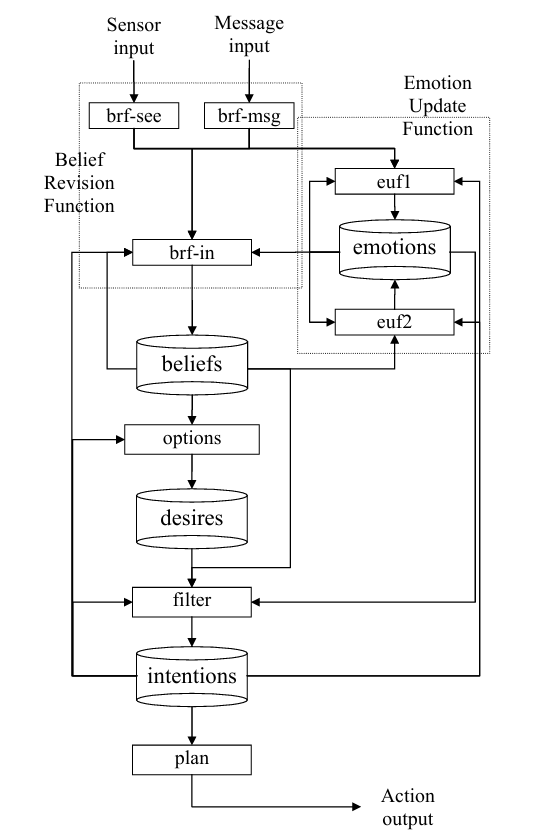
\includegraphics[width=0.62\textwidth]{figures/ebdi_architechture.png}
    \caption{Arquitectura EBDI para agentes emocionales \cite{jiang2007ebdi}.}
    \label{fig:ebdi_architecture}
\end{figure}

Como se observa en la figura  \ref{fig:ebdi_architecture}, las emociones se incorporan como un componente adicional que influye directamente sobre la selección de objetivos, la priorización de planes y la toma de decisiones. De esta forma, el comportamiento del agente no depende únicamente de procesos racionales, sino también de su estado emocional actual.

La arquitectura EBDI utiliza mecanismos inspirados en teorías de appraisal para generar emociones a partir de eventos percibidos por el agente. Estas emociones pueden clasificarse en emociones primarias y secundarias, dependiendo del nivel de procesamiento cognitivo asociado.

Una de las principales aportaciones de EBDI es la separación entre el mecanismo emocional y el proceso de razonamiento práctico del agente \cite{jiang2007ebdi}. Esta separación permite incorporar distintos modelos emocionales sin modificar el núcleo deliberativo de la arquitectura. Además, el modelo distingue entre emociones primarias y secundarias: las emociones primarias actúan como un mecanismo rápido de priorización de creencias y decisiones en entornos dinámicos o con recursos limitados, mientras que las emociones secundarias refinan el razonamiento cuando existe mayor capacidad deliberativa.

De forma simplificada, el ciclo de funcionamiento de un agente EBDI puede describirse mediante las siguientes etapas:

\begin{enumerate}
    \item Percepción del entorno.
    \item Actualización de creencias.
    \item Evaluación emocional de eventos.
    \item Generación de deseos e intenciones.
    \item Selección de acciones.
\end{enumerate}

Esto permite que el agente no actúe únicamente siguiendo objetivos racionales fijos, sino que pueda modificar prioridades dependiendo de la situación emocional percibida.

\subsection{Arquitectura WASABI}

La arquitectura WASABI destaca especialmente por su orientación hacia humanos virtuales expresivos e interacción social creíble \cite{becker2009wasabi}. El sistema combina razonamiento cognitivo con simulación continua de estados afectivos dentro del espacio PAD, permitiendo representar cambios emocionales continuos durante la interacción.

El artículo utiliza como caso de estudio el humano virtual MAX, evaluado en un escenario interactivo basado en un juego de cartas. Además de emociones primarias relacionadas con respuestas rápidas y expresivas, WASABI incorpora emociones secundarias como esperanza (\textit{hope}), alivio (\textit{relief}) y miedo confirmado (\textit{fears-confirmed}), asociadas a procesos cognitivos más complejos y expectativas futuras.

Según los resultados presentados en el artículo, los usuarios percibían al agente como más coherente durante la interacción cuando las emociones secundarias se combinaban con la simulación emocional continua.

En este modelo, las emociones se representan mediante espacios tridimensionales continuos:

\begin{equation}
E = (P, A, D)
\end{equation}

donde:

\begin{itemize}
    \item $P$ representa Pleasure.
    \item $A$ representa Arousal.
    \item $D$ representa Dominance.
\end{itemize}

A diferencia de EBDI, cuyo objetivo principal es integrar emociones dentro del razonamiento deliberativo de agentes racionales, WASABI se centra especialmente en la expresividad emocional y en la percepción de realismo durante la interacción humano-agente. Esta orientación hacia humanos virtuales hace que WASABI sea especialmente relevante para aplicaciones relacionadas con simulación social, personajes virtuales y sistemas de interacción humano-computador capaces de mantener respuestas afectivas más consistentes durante la interacción.

\subsection{Modelos afectivos modernos}

En los últimos años han surgido nuevas propuestas orientadas a integrar emociones, cognición, memoria y comportamiento social dentro de arquitecturas más flexibles e integradas \cite{alfonso2021affect}.

Muchos de estos modelos buscan combinar mecanismos emocionales con memoria, aprendizaje y adaptación social. El objetivo es superar las limitaciones de arquitecturas más rígidas, donde las emociones suelen representarse mediante conjuntos estáticos o respuestas predefinidas.

Asimismo, investigaciones recientes exploran la utilización de modelos híbridos que combinan representación simbólica, lógica difusa, aprendizaje automático y sistemas probabilísticos para mejorar la simulación emocional en agentes inteligentes.

El auge reciente de asistentes conversacionales y sistemas generativos ha incrementado el interés por arquitecturas capaces de representar estados afectivos de manera más flexible y dinámica.

\subsection{Comparación entre arquitecturas}

Las distintas arquitecturas emocionales presentan enfoques diferentes respecto a la representación emocional, el razonamiento afectivo y la toma de decisiones.

\begin{table}[H]
\centering
\caption{Comparación entre arquitecturas emocionales}
\small
\begin{tabular}{|l|l|l|l|}
\hline
\textbf{Arquitectura} & \textbf{Modelo} & \textbf{Representación} & \textbf{Aplicaciones} \\ \hline
BDI & No emocional & Simbólica & Agentes racionales \\ \hline
EBDI & Appraisal & Modular / dependiente del modelo & Agentes deliberativos \\ \hline
WASABI & PAD & Dimensional continua & Humanos virtuales \\ \hline
Modelos modernos & Híbrido & Mixta & IA social avanzada \\ \hline
\end{tabular}
\label{tab:comparacion}
\end{table}

Cada arquitectura presenta ventajas y limitaciones dependiendo del tipo de aplicación y del nivel de complejidad emocional requerido. Mientras que modelos discretos como OCC facilitan la interpretación semántica de emociones específicas, los enfoques dimensionales permiten representar transiciones emocionales más suaves y dinámicas.

Actualmente, la tendencia principal en computación afectiva consiste en desarrollar arquitecturas híbridas capaces de integrar razonamiento cognitivo, representación emocional continua y adaptación social dentro de sistemas inteligentes complejos.